% Options for packages loaded elsewhere
\PassOptionsToPackage{unicode}{hyperref}
\PassOptionsToPackage{hyphens}{url}
%
\documentclass[
]{article}
\usepackage{lmodern}
\usepackage{amssymb,amsmath}
\usepackage{ifxetex,ifluatex}
\ifnum 0\ifxetex 1\fi\ifluatex 1\fi=0 % if pdftex
  \usepackage[T1]{fontenc}
  \usepackage[utf8]{inputenc}
  \usepackage{textcomp} % provide euro and other symbols
\else % if luatex or xetex
  \usepackage{unicode-math}
  \defaultfontfeatures{Scale=MatchLowercase}
  \defaultfontfeatures[\rmfamily]{Ligatures=TeX,Scale=1}
\fi
% Use upquote if available, for straight quotes in verbatim environments
\IfFileExists{upquote.sty}{\usepackage{upquote}}{}
\IfFileExists{microtype.sty}{% use microtype if available
  \usepackage[]{microtype}
  \UseMicrotypeSet[protrusion]{basicmath} % disable protrusion for tt fonts
}{}
\makeatletter
\@ifundefined{KOMAClassName}{% if non-KOMA class
  \IfFileExists{parskip.sty}{%
    \usepackage{parskip}
  }{% else
    \setlength{\parindent}{0pt}
    \setlength{\parskip}{6pt plus 2pt minus 1pt}}
}{% if KOMA class
  \KOMAoptions{parskip=half}}
\makeatother
\usepackage{xcolor}
\IfFileExists{xurl.sty}{\usepackage{xurl}}{} % add URL line breaks if available
\IfFileExists{bookmark.sty}{\usepackage{bookmark}}{\usepackage{hyperref}}
\hypersetup{
  pdftitle={MBD - Estadística - Práctica 1a (ML)},
  pdfauthor={Arturo Menchaca y Víctor Juez},
  hidelinks,
  pdfcreator={LaTeX via pandoc}}
\urlstyle{same} % disable monospaced font for URLs
\usepackage[margin=1in]{geometry}
\usepackage{graphicx,grffile}
\makeatletter
\def\maxwidth{\ifdim\Gin@nat@width>\linewidth\linewidth\else\Gin@nat@width\fi}
\def\maxheight{\ifdim\Gin@nat@height>\textheight\textheight\else\Gin@nat@height\fi}
\makeatother
% Scale images if necessary, so that they will not overflow the page
% margins by default, and it is still possible to overwrite the defaults
% using explicit options in \includegraphics[width, height, ...]{}
\setkeys{Gin}{width=\maxwidth,height=\maxheight,keepaspectratio}
% Set default figure placement to htbp
\makeatletter
\def\fps@figure{htbp}
\makeatother
\setlength{\emergencystretch}{3em} % prevent overfull lines
\providecommand{\tightlist}{%
  \setlength{\itemsep}{0pt}\setlength{\parskip}{0pt}}
\setcounter{secnumdepth}{-\maxdimen} % remove section numbering

\title{MBD - Estadística - Práctica 1a (ML)}
\author{Arturo Menchaca y Víctor Juez}
\date{Noviember 22, 2020}

\begin{document}
\maketitle

\hypertarget{anuxe1lisis-de-variables}{%
\section{Análisis de variables}\label{anuxe1lisis-de-variables}}

El conjunto de datos consta de las siguientes variables:

\begin{itemize}
\tightlist
\item
  id: identificador de la franja horaria (no guarda relación con el
  orden temporal)
\item
  year: año (2011 o 2012)
\item
  hour: hora del día (0 a 23)
\item
  season: 1 = invierno, 2 =primavera, 3 = verano, 4 = otoño
\item
  holiday: si el día era festivo
\item
  workingday: si el día era laborable (ni festivo ni fin de semana)
\item
  weather: cuatro categorías (1 a 4) que van de mejor a peor tiempo
\item
  temp: temperatura en grados celsius
\item
  atemp: sensación de temperatura en grados celsius
\item
  humidity: humedad relativa
\item
  windspeed: velocidad del viento (km/h)
\item
  count (sólo en el conjunto de entrenamiento): número total de
  alquileres en esa franja
\end{itemize}

A continuación mostramos la descriptiva de los datos:

\begin{verbatim}
##    year           hour       season   holiday  workingday weather 
##  2011:3879   Min.   : 0.00   1:1901   0:7466   0:2481     1:5122  
##  2012:3810   1st Qu.: 6.00   2:1920   1: 223   1:5208     2:1981  
##              Median :12.00   3:1943                       3: 586  
##              Mean   :11.57   4:1925                               
##              3rd Qu.:18.00                                        
##              Max.   :23.00                                        
##       temp           atemp          humidity        windspeed     
##  Min.   : 0.82   Min.   : 0.76   Min.   :  0.00   Min.   : 0.000  
##  1st Qu.:13.94   1st Qu.:16.66   1st Qu.: 46.00   1st Qu.: 7.002  
##  Median :20.50   Median :24.24   Median : 62.00   Median :12.998  
##  Mean   :20.27   Mean   :23.70   Mean   : 61.77   Mean   :12.802  
##  3rd Qu.:26.24   3rd Qu.:31.06   3rd Qu.: 77.00   3rd Qu.:16.998  
##  Max.   :41.00   Max.   :45.45   Max.   :100.00   Max.   :56.997  
##      count      
##  Min.   :  1.0  
##  1st Qu.: 41.0  
##  Median :145.0  
##  Mean   :191.4  
##  3rd Qu.:283.0  
##  Max.   :977.0
\end{verbatim}

\hypertarget{categorizaciuxf3n-de-la-variable-hora}{%
\subsection{Categorización de la variable
hora}\label{categorizaciuxf3n-de-la-variable-hora}}

Descriptiva de la variable respuesta en función de la variable hora:

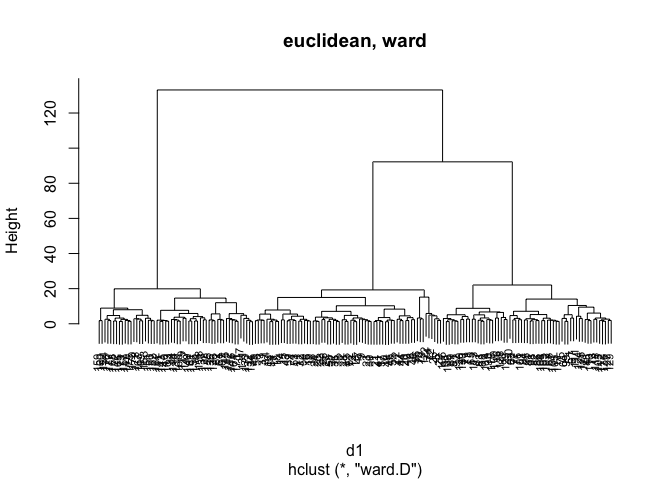
\includegraphics{informe_files/figure-latex/unnamed-chunk-4-1.pdf}

Decidimos agrupar la variable hora en los siguientes grupos:

\begin{itemize}
\tightlist
\item
  Morning: de 0:00h a 6:00h
\item
  Moving: de 6:00h a 8:00h y de 16:00 a 19:00
\item
  Worktime: de 8:00h a 16:00h
\item
  Night: de 19:00h a 23:00h
\end{itemize}

A continuación la descriptiva de la variable hora categorizada:

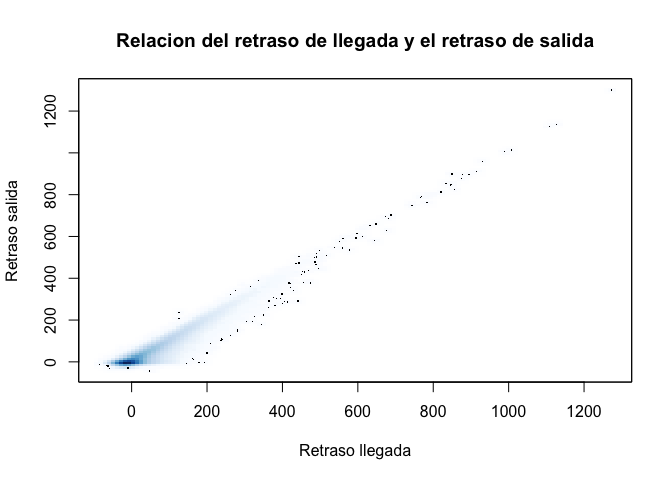
\includegraphics{informe_files/figure-latex/unnamed-chunk-5-1.pdf}

\hypertarget{descriptiva-de-las-variables-numericas}{%
\subsection{Descriptiva de las variables
numericas}\label{descriptiva-de-las-variables-numericas}}

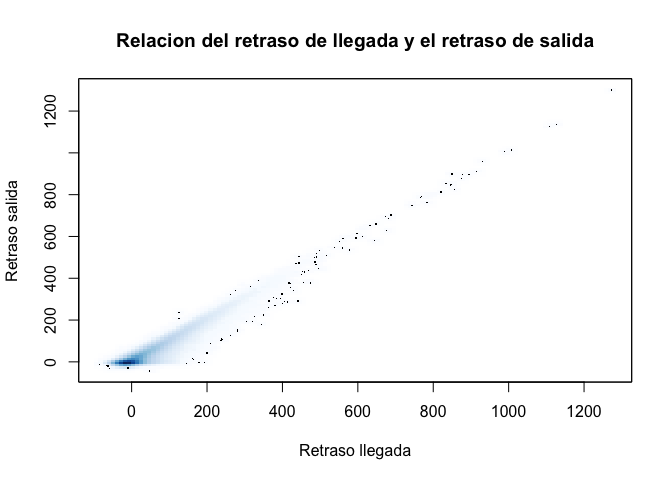
\includegraphics{informe_files/figure-latex/unnamed-chunk-6-1.pdf}

Como podemos observar en la descriptiva que mostramos a arriba, vemos
que la variable temp y atemp estan muy relacionadas, así que vamos a
analizar cual de las dos predice peor la respuesta para descartarla.

\hypertarget{analisis-de-la-variable-temp}{%
\subsubsection{Analisis de la variable
Temp:}\label{analisis-de-la-variable-temp}}

\begin{verbatim}
## 
## Call:
## lm(formula = count ~ temp, data = datos)
## 
## Residuals:
##     Min      1Q  Median      3Q     Max 
## -293.73 -112.49  -32.32   79.01  741.84 
## 
## Coefficients:
##             Estimate Std. Error t value Pr(>|t|)    
## (Intercept)   4.0011     5.2937   0.756     0.45    
## temp          9.2474     0.2437  37.950   <2e-16 ***
## ---
## Signif. codes:  0 '***' 0.001 '**' 0.01 '*' 0.05 '.' 0.1 ' ' 1
## 
## Residual standard error: 167.2 on 7687 degrees of freedom
## Multiple R-squared:  0.1578,   Adjusted R-squared:  0.1577 
## F-statistic:  1440 on 1 and 7687 DF,  p-value: < 2.2e-16
\end{verbatim}

\hypertarget{analisis-de-la-variable-atemp}{%
\subsubsection{Analisis de la variable
Atemp:}\label{analisis-de-la-variable-atemp}}

\begin{verbatim}
## 
## Call:
## lm(formula = count ~ atemp, data = datos)
## 
## Residuals:
##     Min      1Q  Median      3Q     Max 
## -297.99 -113.88  -33.36   80.77  740.65 
## 
## Coefficients:
##             Estimate Std. Error t value Pr(>|t|)    
## (Intercept)  -7.3044     5.6520  -1.292    0.196    
## atemp         8.3862     0.2245  37.360   <2e-16 ***
## ---
## Signif. codes:  0 '***' 0.001 '**' 0.01 '*' 0.05 '.' 0.1 ' ' 1
## 
## Residual standard error: 167.6 on 7687 degrees of freedom
## Multiple R-squared:  0.1537,   Adjusted R-squared:  0.1536 
## F-statistic:  1396 on 1 and 7687 DF,  p-value: < 2.2e-16
\end{verbatim}

Dados los resultados, eliminamos la variable Atemp ya que predice peor
el resultado (PONER RESULTADOS)

\hypertarget{variables-categoricas}{%
\subsection{Variables categoricas}\label{variables-categoricas}}

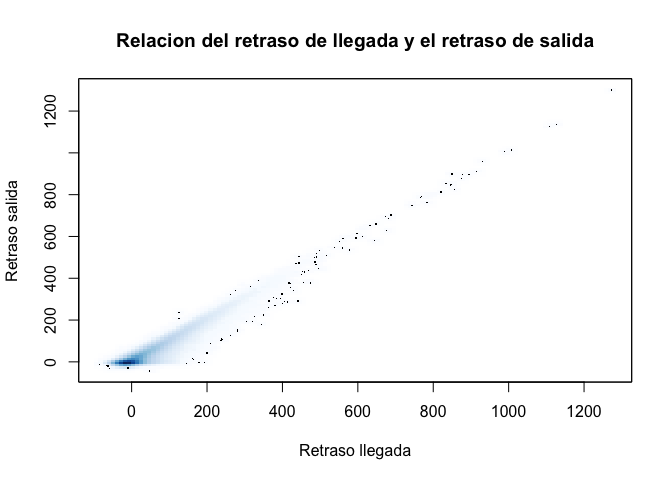
\includegraphics{informe_files/figure-latex/unnamed-chunk-9-1.pdf}

\end{document}
